\documentclass[12pt]{article}
\newcommand\tab[1][1cm]{\hspace*{#1}}
\usepackage{geometry}
\usepackage{graphicx}
\usepackage{fancyhdr}
\usepackage{lastpage}
\usepackage{mathtools}
\usepackage{amssymb}
\usepackage{amsmath}
\pagestyle{fancy}
\fancyhf{}
\renewcommand{\headrulewidth}{0pt}
\cfoot{\thepage \hspace{1pt} of \pageref{LastPage}}
\fancypagestyle{titlepagestyle}
{
   \fancyhf{}
   \cfoot[C]{\thepage \hspace{1pt} of \pageref{LastPage}}
   \renewcommand{\headrulewidth}{0pt}
}

\geometry{  a4paper,            % scientific thesis standard
            left=3cm,
            right=2cm,
            top=2cm,
            bottom=2cm,
 }

\setlength{\parindent}{1cm}     % paragraph indentation

\begin{document}
\title{
  Virtual Notice Board - Raport \\
  \large Cloud Computing}
\author{Andrieș Ștefania IIIA3, Cioată Matei-Alexandru IIIA1}
\maketitle
\thispagestyle{titlepagestyle}

\section{Descrierea proiectului}
\tab \textbf{Virtual Notice Board} este o platformă dezvoltată special pentru instituțiile de învățământ și ajută la comunicarea mai ușoară dintre profesori, studenți/elevi și administrația școlii. Mai concret, fiecare profesor are anunțuri de făcut pentru materiile sale și este mai ușor pentru studenți să găsească aceste informații în același loc decât să verifice zilnic mai multe site-uri. Anunțurile pot fi citite, dar și ascultate în format MP3, indiferent de formatul încărcării inițiale, datorită unor servicii cloud. Studenții pot posta răspunsuri și comentarii la mesajele profesorilor. Atât conturile studentilor cât și cele ale dascălilor sunt create de către administrația instituției. Fiecare persoană va avea acces de la început doar la anunțurile materiilor destinate acesteia (este înscris sau predă).

\section{Studiu de caz raportat la realitatea națională și internațională}
\tab În prezent, având în vedere desfășurarea acestei pandemii, se întâlnesc foarte des cazuri de slabă comunicare între elevi și profesori. Poate fi vorba fie de defecțiuni la serverele instituției , fie de existența prea multor platforme care pot fi dificil de utilizat de toată lumea. Este greu pentru un profesor să selecteze o metodă de predare și examinare online astfel încât să se asigure că informația lui este distribuită tuturor. Totodată, este greu și pentru studenți să se obișnuiască cu câte o platformă și o modalitate diferită la fiecare materie. \\
\tab Așadar, aplicația \textbf{Virtual Notice Board} ajută la continuarea învățării eficiente în această perioadă și nu numai. Toate anunțurile importante ajung în același loc, fiind mai ușor pentru studenți, iar datorită faptului că aceștia sunt notificați în legătură cu folosirea și existența platformei de către administrația instituției de învătământ, profesorii pot fi asigurați că noutățile ajung la toată lumea. Pentru acomodarea profesorilor și elevilor cu aplicația, li se vor oferi tutoriale gratuite și bine explicate.\\
\tab Aplicația poate fi utilă și după încheierea acestei pandemii. Chiar și cu desfășurarea orelor în mod normal, încă se fac anunțuri online.

\section{Soluții asemănătoare - Google Classroom}
\tab \textbf{Google Classroom} este o aplicație cu un scop asemănător: ajută școlile să creeze și să distribuie anunțuri și fișiere și să evalueze studenții în mediul online. Este dezvoltată de Google și este gratuită.\\
\tab \textbf{Google Classroom} combină Google Drive (pentru stocarea de fișiere), Google Docs și Google Slides (pentru scriere). Autentificarea și comunicarea se realizează prin Gmail. Pentru stabilirea deadline-urilor temelor se folosește Google Calendar. Fiecare curs o să aibă un folder separat în care vor apărea fișierele încărcate de utilizator. \\
\tab Studenții se înregistrează la cursuri printr-un cod care le este comunicat de către profesor. După înscriere, este permisă comunicarea student-profesor și student-student. \\
\tab Un mare avantaj al aplicației \textbf{Virtual Notice Board} este faptul că administratorii vor crea de dinainte conturile studenților și profesorilor. Conducerea instituției și secretariatul se vor ocupa de asignarea studenților la materiile la care sunt înscriși, respectiv a profesorilor la cele pe care le predau. Când începe un nou an sau un nou semestru, tot administrația se va ocupa de actualizarea informațiilor (schimbarea materiilor la care studenții sunt înscriși, crearea de noi conturi pentru studenți / profesori nou veniți). Anunțurile postate vor fi convertite automat din text în audio sau invers la adăugare, astfel încât utilizatorii să se informeze în modul dorit. \\
\tab \textbf{Google Classroom} forțează profesorii își organizeze singuri cursurile și să aibă grijă ca fiecare student să obțină codul și să se înscrie pe platformă. În momentul în care se încheie un semestru/an va fi necesară crearea unor noi curs. Totuși \textbf{Google Classroom} are un număr considerabil de avantaje, printre care: alternativa de a rula pe mai multe platforme (web, Android, iOS), opțiunea de a programa deadline-uri pentru teme, posibilitatea întocmirii unui raport de originalitate pentru o lucrare, ajutând astfel atât studenții cât și profesorii, etc..

\section{Tehnologii și servicii utilizate}
\tab Pentru acest proiect vom folosi limbajul de programare \textbf{Python}, versiunea \textbf{3.8}, împreună cu framework-ul \textbf{Flask} pentru dezvoltarea mai rapidă și mai calitativă a aplicațiilor web. Interfața va fi realizată cu ajutorul limbajelor \textbf{HTML} și \textbf{CSS}, întrucât nu este una foarte complexă (nu este formată din foarte multe elemente). \\
Am ales să folosim următoarele servicii de pe \textbf{Google Cloud} (respectiv \textbf{Firebase}):
\begin{itemize}
	\item \textbf{Firebase Authentication} este un serviciu foarte potrivit pentru această aplicație. Autentificarea se realizează cu un e-mail creat pe orice platformă (Gmail, Yahoo sau chiar e-mail-ul facultății/școlii). Utilizatorii au posilibitatea să își confirme e-mail-ul și să își schimbe parola, care este păstrată mereu secretă de acest serviciu.
	\item \textbf{Firebase Storage} este un serviciu ce permite stocarea fișierelor cu anunțuri încărcate de profesori în format text și MP3. Vom organiza documentele astfel încât doar anumiți studenți și profesori să le poată vizualiza, descărca sau șterge. 
	\item \textbf{Text-to-Speech} și \textbf{Speech-to-Text} ajută la conversia fișierelor încărcate. Un fișier text va fi automat încărcat și în format audio și invers.
	\item \textbf{Datastore} va stoca date despre utilizatori (dacă este student, profesor sau administrator, materiile la care este înscris sau pe care le predă, etc..). De asemenea, într-o tabelă separată vor fi stocate căile fișierelor cu anunțuri din storage, împreună cu token-urile de acces.
	\item \textbf{Cloud Function} este rulată la ștergerea unei înregistrări din baza de date. În momentul în care un utilizator optează să șteargă un anunț dintr-un anumit format, funcția va curața și perechea sa atât din storage cât și din baza de date.
\end{itemize}

\section{Business Model Canvas}
\begin{figure}[h!]
	\centering
    	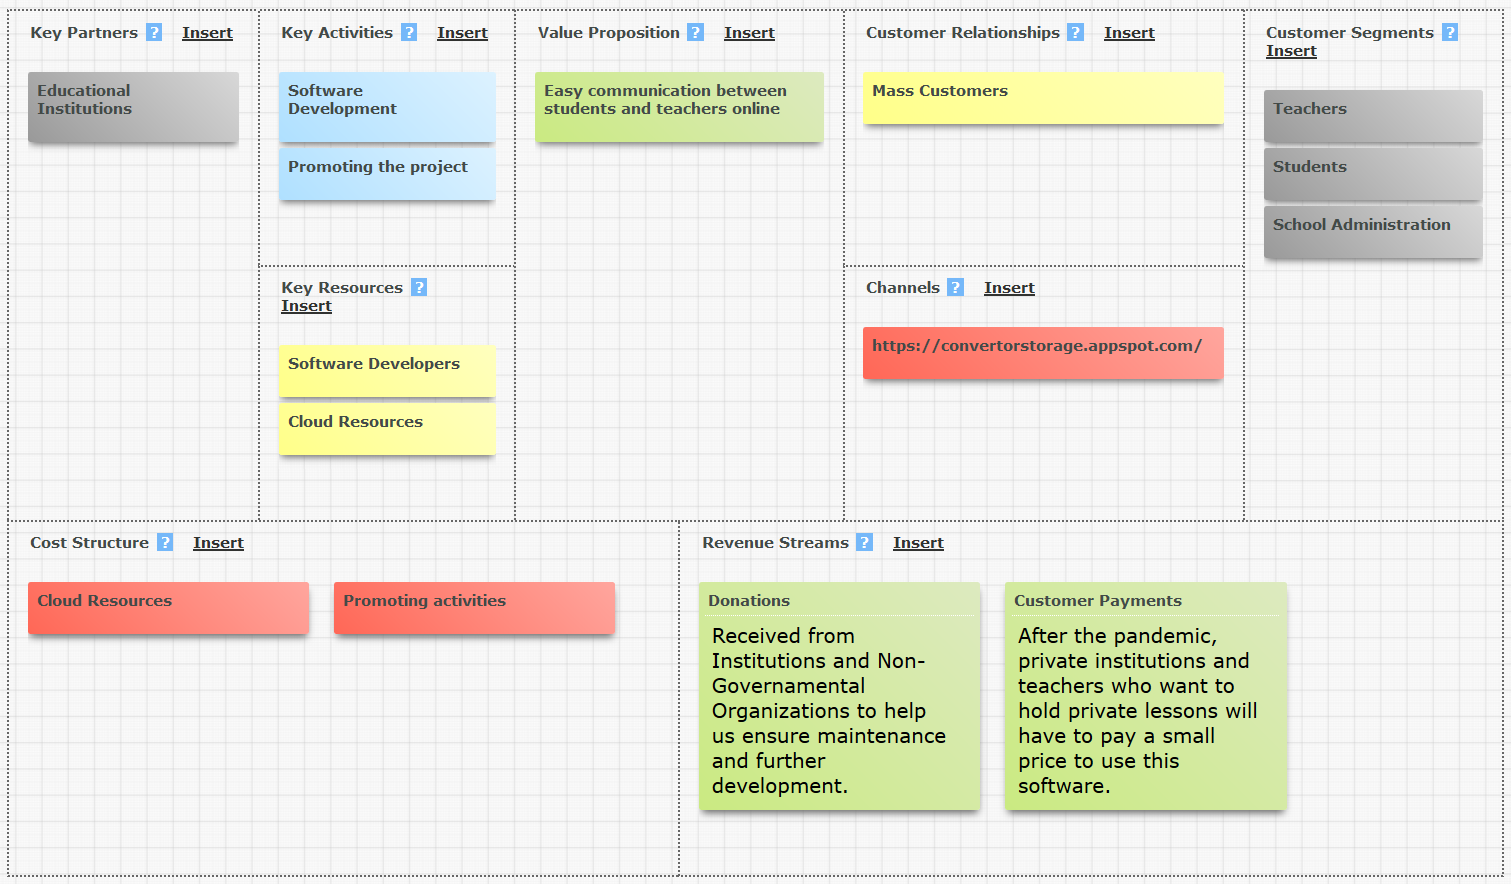
\includegraphics[width=0.95\textwidth]{businessCanvas.png}
        \caption{Business Model Canvas for \textbf{Virtual Notice Board}}
\end{figure}

\section{Diagramă Use-Case}
\begin{figure}[h!]
	\centering
    	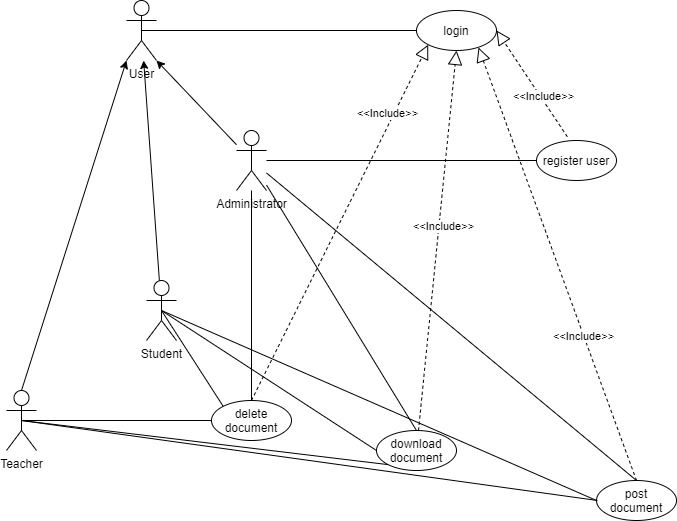
\includegraphics[width=0.85\textwidth]{use_case.jpg}
        \caption{Diagramă Use-Case}
\end{figure}

\section{Diagramă arhitecturală}
\begin{figure}[h!]
	\centering
    	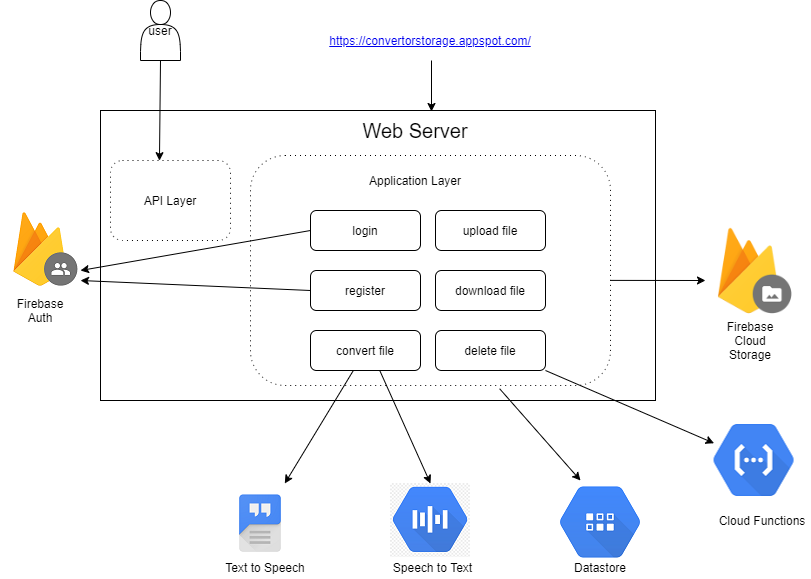
\includegraphics[width=1.0\textwidth]{architectural.png}
        \caption{Diagramă arhitecturală}
\end{figure}

\end{document}